% GNUPLOT: LaTeX picture with Postscript
\begingroup
  \makeatletter
  \providecommand\color[2][]{%
    \GenericError{(gnuplot) \space\space\space\@spaces}{%
      Package color not loaded in conjunction with
      terminal option `colourtext'%
    }{See the gnuplot documentation for explanation.%
    }{Either use 'blacktext' in gnuplot or load the package
      color.sty in LaTeX.}%
    \renewcommand\color[2][]{}%
  }%
  \providecommand\includegraphics[2][]{%
    \GenericError{(gnuplot) \space\space\space\@spaces}{%
      Package graphicx or graphics not loaded%
    }{See the gnuplot documentation for explanation.%
    }{The gnuplot epslatex terminal needs graphicx.sty or graphics.sty.}%
    \renewcommand\includegraphics[2][]{}%
  }%
  \providecommand\rotatebox[2]{#2}%
  \@ifundefined{ifGPcolor}{%
    \newif\ifGPcolor
    \GPcolortrue
  }{}%
  \@ifundefined{ifGPblacktext}{%
    \newif\ifGPblacktext
    \GPblacktexttrue
  }{}%
  % define a \g@addto@macro without @ in the name:
  \let\gplgaddtomacro\g@addto@macro
  % define empty templates for all commands taking text:
  \gdef\gplbacktext{}%
  \gdef\gplfronttext{}%
  \makeatother
  \ifGPblacktext
    % no textcolor at all
    \def\colorrgb#1{}%
    \def\colorgray#1{}%
  \else
    % gray or color?
    \ifGPcolor
      \def\colorrgb#1{\color[rgb]{#1}}%
      \def\colorgray#1{\color[gray]{#1}}%
      \expandafter\def\csname LTw\endcsname{\color{white}}%
      \expandafter\def\csname LTb\endcsname{\color{black}}%
      \expandafter\def\csname LTa\endcsname{\color{black}}%
      \expandafter\def\csname LT0\endcsname{\color[rgb]{1,0,0}}%
      \expandafter\def\csname LT1\endcsname{\color[rgb]{0,1,0}}%
      \expandafter\def\csname LT2\endcsname{\color[rgb]{0,0,1}}%
      \expandafter\def\csname LT3\endcsname{\color[rgb]{1,0,1}}%
      \expandafter\def\csname LT4\endcsname{\color[rgb]{0,1,1}}%
      \expandafter\def\csname LT5\endcsname{\color[rgb]{1,1,0}}%
      \expandafter\def\csname LT6\endcsname{\color[rgb]{0,0,0}}%
      \expandafter\def\csname LT7\endcsname{\color[rgb]{1,0.3,0}}%
      \expandafter\def\csname LT8\endcsname{\color[rgb]{0.5,0.5,0.5}}%
    \else
      % gray
      \def\colorrgb#1{\color{black}}%
      \def\colorgray#1{\color[gray]{#1}}%
      \expandafter\def\csname LTw\endcsname{\color{white}}%
      \expandafter\def\csname LTb\endcsname{\color{black}}%
      \expandafter\def\csname LTa\endcsname{\color{black}}%
      \expandafter\def\csname LT0\endcsname{\color{black}}%
      \expandafter\def\csname LT1\endcsname{\color{black}}%
      \expandafter\def\csname LT2\endcsname{\color{black}}%
      \expandafter\def\csname LT3\endcsname{\color{black}}%
      \expandafter\def\csname LT4\endcsname{\color{black}}%
      \expandafter\def\csname LT5\endcsname{\color{black}}%
      \expandafter\def\csname LT6\endcsname{\color{black}}%
      \expandafter\def\csname LT7\endcsname{\color{black}}%
      \expandafter\def\csname LT8\endcsname{\color{black}}%
    \fi
  \fi
    \setlength{\unitlength}{0.0500bp}%
    \ifx\gptboxheight\undefined%
      \newlength{\gptboxheight}%
      \newlength{\gptboxwidth}%
      \newsavebox{\gptboxtext}%
    \fi%
    \setlength{\fboxrule}{0.5pt}%
    \setlength{\fboxsep}{1pt}%
    \definecolor{tbcol}{rgb}{1,1,1}%
\begin{picture}(9060.00,7920.00)%
    \gplgaddtomacro\gplbacktext{%
      \csname LTb\endcsname%%
      \put(625,5619){\makebox(0,0)[r]{\strut{}-75}}%
      \csname LTb\endcsname%%
      \put(625,6047){\makebox(0,0)[r]{\strut{}-60}}%
      \csname LTb\endcsname%%
      \put(625,6474){\makebox(0,0)[r]{\strut{}-45}}%
      \csname LTb\endcsname%%
      \put(625,6902){\makebox(0,0)[r]{\strut{}-30}}%
      \csname LTb\endcsname%%
      \put(625,7329){\makebox(0,0)[r]{\strut{}-15}}%
      \csname LTb\endcsname%%
      \put(625,7757){\makebox(0,0)[r]{\strut{}0}}%
      \csname LTb\endcsname%%
      \put(1027,5301){\makebox(0,0){\strut{}}}%
      \csname LTb\endcsname%%
      \put(1789,5301){\makebox(0,0){\strut{}}}%
      \csname LTb\endcsname%%
      \put(2551,5301){\makebox(0,0){\strut{}}}%
      \csname LTb\endcsname%%
      \put(3312,5301){\makebox(0,0){\strut{}}}%
      \csname LTb\endcsname%%
      \put(4074,5301){\makebox(0,0){\strut{}}}%
      \csname LTb\endcsname%%
      \put(4836,5301){\makebox(0,0){\strut{}}}%
      \csname LTb\endcsname%%
      \put(2779,5719){\makebox(0,0){\strut{}DBS Opposing}}%
    }%
    \gplgaddtomacro\gplfronttext{%
      \csname LTb\endcsname%%
      \put(4080,6470){\makebox(0,0)[r]{\strut{}$\mathrm{CH}_2$}}%
      \csname LTb\endcsname%%
      \put(4080,6207){\makebox(0,0)[r]{\strut{}$\mathrm{NH}_3$}}%
      \csname LTb\endcsname%%
      \put(4080,5943){\makebox(0,0)[r]{\strut{}$\mathrm{H}_2\mathrm{O}$}}%
      \csname LTb\endcsname%%
      \put(4080,5679){\makebox(0,0)[r]{\strut{}$\mathrm{HF}$}}%
      \csname LTb\endcsname%%
      \put(72,6688){\rotatebox{-270.00}{\makebox(0,0){\strut{}Energy (meV)}}}%
    }%
    \gplgaddtomacro\gplbacktext{%
      \csname LTb\endcsname%%
      \put(4828,5477){\makebox(0,0)[r]{\strut{}}}%
      \csname LTb\endcsname%%
      \put(4828,6047){\makebox(0,0)[r]{\strut{}}}%
      \csname LTb\endcsname%%
      \put(4828,6617){\makebox(0,0)[r]{\strut{}}}%
      \csname LTb\endcsname%%
      \put(4828,7187){\makebox(0,0)[r]{\strut{}}}%
      \csname LTb\endcsname%%
      \put(4828,7757){\makebox(0,0)[r]{\strut{}}}%
      \csname LTb\endcsname%%
      \put(5231,5301){\makebox(0,0){\strut{}}}%
      \csname LTb\endcsname%%
      \put(5993,5301){\makebox(0,0){\strut{}}}%
      \csname LTb\endcsname%%
      \put(6754,5301){\makebox(0,0){\strut{}}}%
      \csname LTb\endcsname%%
      \put(7516,5301){\makebox(0,0){\strut{}}}%
      \csname LTb\endcsname%%
      \put(8278,5301){\makebox(0,0){\strut{}}}%
      \csname LTb\endcsname%%
      \put(9039,5301){\makebox(0,0){\strut{}}}%
      \csname LTb\endcsname%%
      \put(6983,5719){\makebox(0,0){\strut{}DBS Parallel}}%
    }%
    \gplgaddtomacro\gplfronttext{%
    }%
    \gplgaddtomacro\gplbacktext{%
      \csname LTb\endcsname%%
      \put(625,2975){\makebox(0,0)[r]{\strut{}-2.6}}%
      \csname LTb\endcsname%%
      \put(625,3379){\makebox(0,0)[r]{\strut{}-2.4}}%
      \csname LTb\endcsname%%
      \put(625,3783){\makebox(0,0)[r]{\strut{}-2.2}}%
      \csname LTb\endcsname%%
      \put(625,4186){\makebox(0,0)[r]{\strut{}-2.0}}%
      \csname LTb\endcsname%%
      \put(625,4590){\makebox(0,0)[r]{\strut{}-1.8}}%
      \csname LTb\endcsname%%
      \put(625,4994){\makebox(0,0)[r]{\strut{}-1.6}}%
      \csname LTb\endcsname%%
      \put(625,5398){\makebox(0,0)[r]{\strut{}-1.4}}%
      \csname LTb\endcsname%%
      \put(1027,2799){\makebox(0,0){\strut{}}}%
      \csname LTb\endcsname%%
      \put(1789,2799){\makebox(0,0){\strut{}}}%
      \csname LTb\endcsname%%
      \put(2551,2799){\makebox(0,0){\strut{}}}%
      \csname LTb\endcsname%%
      \put(3312,2799){\makebox(0,0){\strut{}}}%
      \csname LTb\endcsname%%
      \put(4074,2799){\makebox(0,0){\strut{}}}%
      \csname LTb\endcsname%%
      \put(4836,2799){\makebox(0,0){\strut{}}}%
      \csname LTb\endcsname%%
      \put(2779,3217){\makebox(0,0){\strut{}VBS Opposing}}%
    }%
    \gplgaddtomacro\gplfronttext{%
      \csname LTb\endcsname%%
      \put(72,4186){\rotatebox{-270.00}{\makebox(0,0){\strut{}Energy (eV)}}}%
    }%
    \gplgaddtomacro\gplbacktext{%
      \csname LTb\endcsname%%
      \put(4828,2975){\makebox(0,0)[r]{\strut{}}}%
      \csname LTb\endcsname%%
      \put(4828,3379){\makebox(0,0)[r]{\strut{}}}%
      \csname LTb\endcsname%%
      \put(4828,3783){\makebox(0,0)[r]{\strut{}}}%
      \csname LTb\endcsname%%
      \put(4828,4186){\makebox(0,0)[r]{\strut{}}}%
      \csname LTb\endcsname%%
      \put(4828,4590){\makebox(0,0)[r]{\strut{}}}%
      \csname LTb\endcsname%%
      \put(4828,4994){\makebox(0,0)[r]{\strut{}}}%
      \csname LTb\endcsname%%
      \put(4828,5398){\makebox(0,0)[r]{\strut{}}}%
      \csname LTb\endcsname%%
      \put(5231,2799){\makebox(0,0){\strut{}}}%
      \csname LTb\endcsname%%
      \put(5993,2799){\makebox(0,0){\strut{}}}%
      \csname LTb\endcsname%%
      \put(6754,2799){\makebox(0,0){\strut{}}}%
      \csname LTb\endcsname%%
      \put(7516,2799){\makebox(0,0){\strut{}}}%
      \csname LTb\endcsname%%
      \put(8278,2799){\makebox(0,0){\strut{}}}%
      \csname LTb\endcsname%%
      \put(9039,2799){\makebox(0,0){\strut{}}}%
      \csname LTb\endcsname%%
      \put(6983,3217){\makebox(0,0){\strut{}VBS Parallel}}%
    }%
    \gplgaddtomacro\gplfronttext{%
    }%
    \gplgaddtomacro\gplbacktext{%
      \csname LTb\endcsname%%
      \put(625,474){\makebox(0,0)[r]{\strut{}-8.0}}%
      \csname LTb\endcsname%%
      \put(625,1044){\makebox(0,0)[r]{\strut{}-6.0}}%
      \csname LTb\endcsname%%
      \put(625,1614){\makebox(0,0)[r]{\strut{}-4.0}}%
      \csname LTb\endcsname%%
      \put(625,2184){\makebox(0,0)[r]{\strut{}-2.0}}%
      \csname LTb\endcsname%%
      \put(625,2754){\makebox(0,0)[r]{\strut{}0.0}}%
      \csname LTb\endcsname%%
      \put(1027,298){\makebox(0,0){\strut{}$5$}}%
      \csname LTb\endcsname%%
      \put(1789,298){\makebox(0,0){\strut{}$10$}}%
      \csname LTb\endcsname%%
      \put(2551,298){\makebox(0,0){\strut{}$15$}}%
      \csname LTb\endcsname%%
      \put(3312,298){\makebox(0,0){\strut{}$20$}}%
      \csname LTb\endcsname%%
      \put(4074,298){\makebox(0,0){\strut{}$25$}}%
      \csname LTb\endcsname%%
      \put(4836,298){\makebox(0,0){\strut{}$30$}}%
      \csname LTb\endcsname%%
      \put(2779,716){\makebox(0,0){\strut{}Interaction Energy Opposing}}%
    }%
    \gplgaddtomacro\gplfronttext{%
      \csname LTb\endcsname%%
      \put(72,1685){\rotatebox{-270.00}{\makebox(0,0){\strut{}Energy (meV)}}}%
      \csname LTb\endcsname%%
      \put(2779,34){\makebox(0,0){\strut{}Distance (\AA)}}%
    }%
    \gplgaddtomacro\gplbacktext{%
      \csname LTb\endcsname%%
      \put(4828,474){\makebox(0,0)[r]{\strut{}}}%
      \csname LTb\endcsname%%
      \put(4828,1044){\makebox(0,0)[r]{\strut{}}}%
      \csname LTb\endcsname%%
      \put(4828,1614){\makebox(0,0)[r]{\strut{}}}%
      \csname LTb\endcsname%%
      \put(4828,2184){\makebox(0,0)[r]{\strut{}}}%
      \csname LTb\endcsname%%
      \put(4828,2754){\makebox(0,0)[r]{\strut{}}}%
      \csname LTb\endcsname%%
      \put(5231,298){\makebox(0,0){\strut{}$5$}}%
      \csname LTb\endcsname%%
      \put(5993,298){\makebox(0,0){\strut{}$10$}}%
      \csname LTb\endcsname%%
      \put(6754,298){\makebox(0,0){\strut{}$15$}}%
      \csname LTb\endcsname%%
      \put(7516,298){\makebox(0,0){\strut{}$20$}}%
      \csname LTb\endcsname%%
      \put(8278,298){\makebox(0,0){\strut{}$25$}}%
      \csname LTb\endcsname%%
      \put(9039,298){\makebox(0,0){\strut{}$30$}}%
      \csname LTb\endcsname%%
      \put(6983,716){\makebox(0,0){\strut{}Interaction Energy Parallel}}%
    }%
    \gplgaddtomacro\gplfronttext{%
      \csname LTb\endcsname%%
      \put(6983,34){\makebox(0,0){\strut{}Distance (\AA)}}%
    }%
    \gplbacktext
    \put(0,0){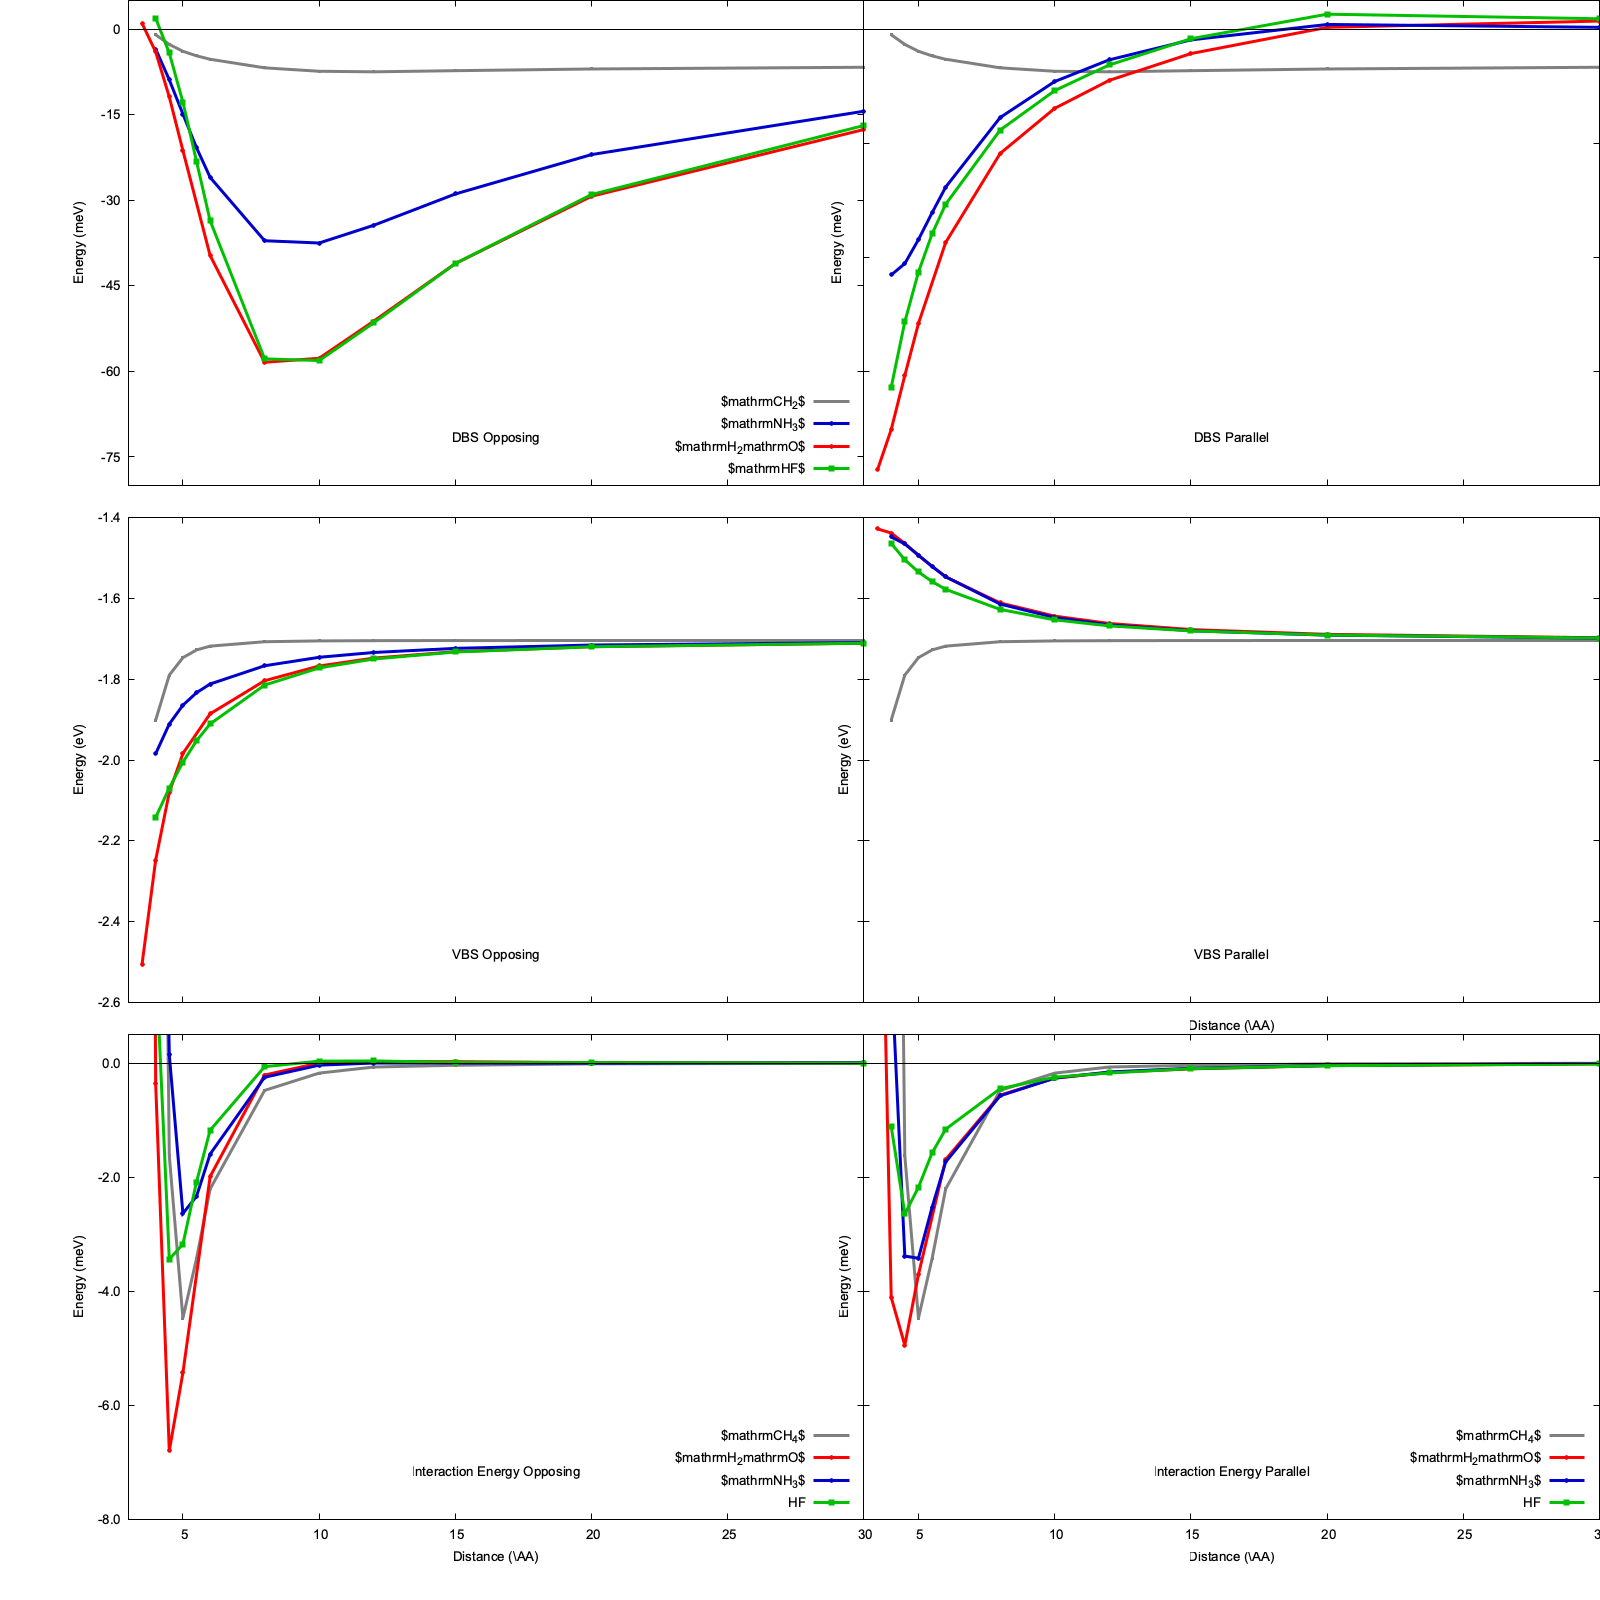
\includegraphics[width={453.00bp},height={396.00bp}]{chapters/results/image/scan_all}}%
    \gplfronttext
  \end{picture}%
\endgroup
